\section{Análise dos Resultados e Conclusão}
Neste capítulo apresentaremos a comparação entre o tempo de execução dos algoritmos de ordenação e as concluções gerais sobre o projeto.

Na Tabela~\ref{tab:complexidade} podemos ver a complexidade dos algoritmos utilizados, como as
\renewcommand{\arraystretch}{1.5}
  \begin{table}[h]
    \centering
    \begin{tabular}[h]{|l|c|c|c|} \hline
      Algoritmo & Melhor caso & Caso Médio & Pior caso \\ \hline
      Bubble Sort & $\Omega(n^2)$ & $\Theta(n^2)$ & $O(n^2)$ \\ \hline
      Bubble Sort com otimização& $\Omega(n)$ & $\Theta(n^2)$ & $O(n^2)$ \\ \hline
      Insertion Sort & $\Omega(n)$ & $\Theta(n^2)$ & $O(n^2)$ \\ \hline
      Selection Sort & $\Omega(n^2)$ & $\Theta(n^2)$ & $O(n^2)$ \\ \hline
      Merge Sort & $\Omega(nlog(n))$ & $\Theta(nlog(n))$ & $O(nlog(n))$ \\ \hline
      Heap Sort & $\Omega(nlog(n))$ & $\Theta(nlog(n))$ & $O(nlog(n))$ \\ \hline
      Quick Sort & $\Omega(nlog(n))$ & $\Theta(nlog(n))$ & $O(n^2)$ \\ \hline
      Busca Binária & $\Omega(1)$ & $\Theta(log(n))$ & $O(log(n))$ \\ \hline
      Busca do Subvetor Máximo & $\Omega(nlog(n))$ & $\Theta(nlog(n))$ & $O(nlog(n))$ \\ \hline
    \end{tabular}
    \caption{Complexidade dos algoritmos analisados}
    \label{tab:complexidade}
  \end{table}
  entradas geradas para os problemas possuiam valores aleatórios, esperava-se que os algoritmos executassem para o caso médio, como foi para a maioria dos casos testados, entretanto o Insertion Sort executou com comportamento $nlog(n)$, variando entre o pior e o melhor caso, pois como a entrada continha diversos elementos repetidos, era possível encontrar com facilidade a posição correta para a inserção dos elementos.

  O Quick Sort, contudo, variou entre o caso médio e o pior caso, com o pivô fixo na última posição e muitos valores repetidos, o algoritmo não se mostrou eficiente durante a fase do particionamento, gerando uma árvore de recursão desbalanceada, porém ele ainda se mostrou mais eficiente que os algoritmos que executam em $n^2$.

  Para o algoritmo de Busca Binária, o fator da repetição dos números também influenciou no resultado final, podemos observar o algoritmo apresentando comportamento $\Theta(1)$. Mesmo quando o algoritmo caiu no seu pior caso, buscar um elemento cujo valor não está contido no vetor, seu tempo de execução continua ótimo, independente do tamanho da entrada.

  Na Figura~\ref{fig:eficientes} podemos ver o comparativo entre os tempos de execução dos algoritmos de ordenação que se mostraram mais eficientes na resolução do problema,
\begin{figure}[ht]
\centering
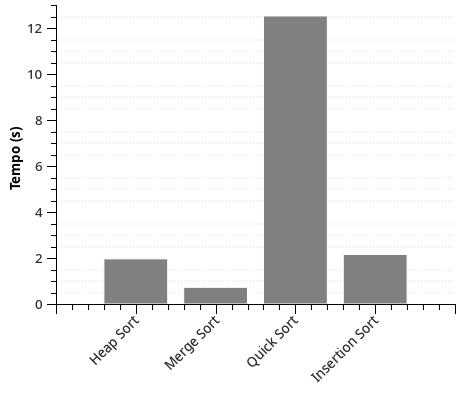
\includegraphics[scale=0.9]{images/eficientes_graph.jpg}
\caption{Algoritmos eficientes durante a análise empírica}
\label{fig:eficientes}
\end{figure}
o Merge Sort se mostrou mais eficiente, seguido pelo Heap Sort e o Insertion Sort, entretanto devemos enfatizar que o Insertion Sort é considerado um algoritmo de ordenação ineficiente, pois como sabemos, um algoritmo tem maior chance de executar com comportamento tendendo ao caso médio e que o caso médio costuma ser tão ruim quanto o pior caso.


Na Figura~\ref{fig:ineficientes} vemos o tempo de execução para os algoritmos ineficientes, 
\begin{figure}[ht]
\centering
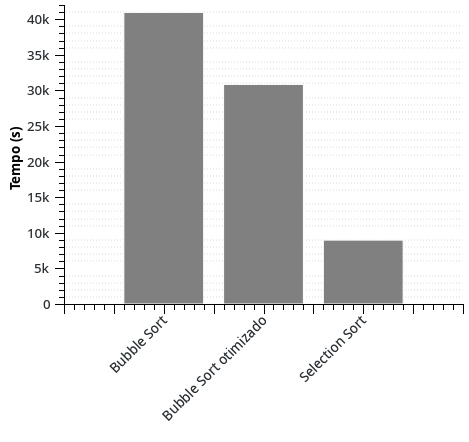
\includegraphics[scale=0.9]{images/ineficientes_graph.jpg}
\caption{Algoritmos ineficientes durante a análise empírica}
\label{fig:ineficientes}
\end{figure}
o Bubble Sort apresentou uma melhora significativa, contudo, ainda longe de tornar o algoritmo utilizável para a resolução de problemas com entradas muito grandes, sendo que a partir de quinhentos mil elementos, ele leva cerca de duas horas para finalizar o processo. O Selection Sort, apesar de realizar o mesmo número de instruções que o Bubble Sort, conseguiu executar em um tempo muito menor.
%%%Local Variables:
%%% TeX-master: "Artigo"
%%% End: